\documentclass[pdf,sprung,slideColor,nocolorBG]{beamer}
%
%\documentclass[hyperref={pdfpagelabels=false}]{beamer}
\mode<presentation>

\newenvironment{colortheme}[1]{
\def\ProvidesPackageRCS $##1${\relax}
\renewcommand{\ProcessOptions}{\relax}
\makeatletter
\input beamercolortheme#1.sty
\makeatother
}{}

\let\Tiny=\tiny
\usetheme{Adelaide}
\usefonttheme[stillsansseriftext]{serif}
\setbeamerfont{structure}{series=\bfseries}
\setbeamertemplate{frametitle}[default][center]
\usepackage[figurename={}]{caption}
\usepackage[latin1]{inputenc}
%\usepackage{amsmath}   %needed for \begin{align}... \end{align} environment
\usepackage{amsfonts}
\usepackage{amssymb}
%\usepackage{amscd}
%\usepackage[all]{xy}
\usepackage{xcolor}
\usepackage{enumerate}
%
\newcommand{\slidecite}[1]{\tiny{(#1)}\normalsize{}}
\newcommand{\smallcite}[1]{\small{(#1)}\normalsize{}}

\newcommand{\mb}[1]{\mathbb{#1}}
\newcommand{\mf}[1]{\mathbf{#1}}
\newcommand{\Emph}[1]{\emph{\textcolor{blue}{#1}}}
\newcommand{\Red}[1]{\mathbf{\textcolor{red}{#1}}}

\newcommand{\abs}[1]{\left| #1 \right|}
\newcommand{\norm}[1]{\left\| #1 \right\|}
\newcommand{\To}{\rightarrow}

\newcommand{\Cay}[1]{\operatorname{Cay}\left(#1\right)}
\newcommand{\Clique}[1]{\omega\left(#1\right)}
\newcommand{\dual}[1]{\widetilde{#1}}
\newcommand{\support}[1]{\operatorname{supp}\left(#1\right)}
\newcommand{\weight}[1]{\operatorname{wt}\left(#1\right)}
\newcommand{\weightclass}[1]{\operatorname{wc}\left(#1\right)}

\newcommand{\F}{\mb{F}}
\newcommand{\G}{\mb{G}}
\newcommand{\R}{\mb{R}}
\newcommand{\Z}{\mb{Z}}
\newtheorem{Def}{Definition}
\newtheorem{Conjecture}{Conjecture}
\newtheorem{Question}{Question}
\newtheorem{Proposition}{Proposition}

\title{Relations between equivalences of bent functions}
\author{Paul Leopardi}

\date{For Australian Mathematical Society Conference 2023}

\institute{Australian National University (professional staff)
\\
ACCESS-NRI}
\titlegraphic{
%\includegraphics[angle=0,width=10mm]{../../common/beamer-anu-colourlogo.png}
%\includegraphics[angle=0,width=20mm]{../../common/carma_logo.jpg}
}
\begin{document}

\frame{\titlepage}

\section{Preliminaries}

\begin{colortheme}{jubata}

\begin{frame}
\frametitle{Motivation}

Question:

~

\Emph{Which strongly regular graphs arise as Cayley graphs of bent Boolean functions?}

\end{frame}
\end{colortheme}

\begin{colortheme}{seagull}

\begin{frame}
\frametitle{Bent functions}
% Bent functions can be defined in a number of equivalent ways.
% The definition used here involves the Walsh Hadamard Transform.
\begin{Def}
\label{def-Walsh-Hadamard-transform}
The Walsh Hadamard transform of
a Boolean function $f : \F_2^{2m} \To \F_2$ is
\begin{align*}
W_f(x)
&:=
\sum_{y \in \F_2^{2m}} (-1)^{f(y) + \langle x, y \rangle}
\end{align*}
\end{Def}

\begin{Def}
\label{def-Bent-function}
A Boolean function $f : \F_2^{2m} \To \F_2$ is \Emph{bent}
if and only if its Walsh Hada\-mard transform has constant absolute value $2^{m}$.
% \cite[p. 74]{Dil74}
% \cite[p. 300]{Rot76}.
\end{Def}
\slidecite{Dillon 1974; Rothaus 1976}
\end{frame}

\begin{frame}
\frametitle{The Cayley graph of a Boolean function}
%\begin{center}
\begin{Def}

The \Emph{Cayley graph} $\Cay{f}$ of a Boolean function

~

\begin{align*}
%
f : \F_2^n \To \F_2 \quad \text{where} \quad f(0) = 0
%
\end{align*}

~

is
an undirected graph with

\begin{align*}
V(\Cay{f}) &:= \F_2^n, \quad (x,y) \in E(\Cay{f}) \Leftrightarrow f(x+y) = 1.
\end{align*}

\end{Def}

\slidecite{Bernasconi and Codenotti 1999}
\end{frame}

\begin{frame}
\frametitle{Strongly regular graphs}
%\begin{center}
\begin{Def}

A simple graph $\Gamma$ of order $v$ is \Emph{strongly regular} with parameters
$(v,k,\lambda,\mu)$ if

~

\begin{itemize}
 \item
each vertex has degree $k,$

~
 \item
each adjacent pair of vertices has $\lambda$ common neighbours, and

~
\item
each nonadjacent pair of vertices has $\mu$ common neighbours.
\end{itemize}

\end{Def}

~

~

\slidecite{Brouwer, Cohen and Neumaier 1989}

%\end{center}
\end{frame}

\begin{frame}
\frametitle{Cayley graphs of bent functions}

\begin{Proposition}
\smallcite{Bernasconi and Codenotti 1999}

The Cayley graph $\Cay{f}$ of a bent function $f$ on $\F_2^{2m}$

with $f(0)=0$ is a strongly regular graph with $\lambda = \mu.$
\end{Proposition}

The parameters of $\Cay{f}$ are
\begin{align*}
(v,k,\lambda) = &(4^m, 2^{2 m - 1} - 2^{m-1}, 2^{2 m - 2} - 2^{m-1})
\\
  \text{or} \quad &(4^m, 2^{2 m - 1} + 2^{m-1}, 2^{2 m - 2} + 2^{m-1}).
\end{align*}

\slidecite{Bernasconi and Codenotti 1999}
\end{frame}

\end{colortheme}

\section{Equivalence of bent functions}

\begin{colortheme}{seagull}

\begin{frame}
\frametitle{Extended affine equivalence}

\begin{Def}
For bent functions $f,g : \F_2^{2m} \To \F_2$,

$f$ is \Emph{extended affine equivalent} to $g$ if and only if
\begin{align*}
g(x) &= f(A x + b) + \langle c, x \rangle + \delta
\end{align*}
for some $A \in GL(2m,2)$, $b, c \in \F_2^{2m}$, $\delta \in \F_2$.
\end{Def}

~

~

\slidecite{Budaghyan, Carlet and Pott 2006}
\end{frame}

\end{colortheme}

\begin{colortheme}{jubata}

\begin{frame}
\frametitle{General linear equivalence}

\begin{Def}
For bent functions $f,g : \F_2^{2m} \To \F_2$,
$f$ is \Emph{general linear equivalent} to $g$ if and only if
\begin{align*}
g(x) &= f(A x)
\end{align*}
for some $A \in GL(2m,2)$.
\end{Def}
\end{frame}
\begin{frame}
\frametitle{Extended translation equivalence}

\begin{Def}
For bent functions $f,g : \F_2^{2m} \To \F_2$,

$f$ is \Emph{extended translation equivalent} to $g$ if and only if
\begin{align*}
g(x) &= f(x + b) + \langle c, x \rangle + \delta
\end{align*}
for $b, c \in \F_2^{2m}$, $\delta \in \F_2$.
\end{Def}
\end{frame}

\begin{frame}
\frametitle{Cayley equivalence}
\begin{Def}
%
For $f, g : \F_2^{2m} \To \F_2$, with both $f$ and $g$ bent,

we call $f$ and $g$ \Emph{Cayley equivalent},
and write $f \equiv g$,

if and only if $f(0)=g(0)=0$ and $\Cay{f} \equiv \Cay{g}$ as graphs.

~

Equivalently, $f \equiv g$ if and only if $f(0)=g(0)=0$ and

there exists a bijection $\pi : \F_2^{2m} \To \F_2^{2m}$ such that
\begin{align*}
g(x+y) &= f \big(\pi(x)+\pi(y)\big) \quad \text{for all~} x,y \in \F_2^{2m}.
\end{align*}
\end{Def}
\end{frame}
\begin{frame}
\frametitle{Extended Cayley equivalence}
\begin{Def}
For $f, g : \F_2^{2m} \To \F_2$, with both $f$ and $g$ bent,

if there exist $\delta, \epsilon \in \{0,1\}$ such that $f + \delta \equiv g + \epsilon$,

we call $f$ and $g$ \Emph{extended Cayley (EC) equivalent} and write $f \cong g$.
\end{Def}
Extended Cayley equivalence is an equivalence relation on the set of all bent functions on $\F_2^{2m}$.
\end{frame}

\begin{frame}
\frametitle{General linear equivalence \\ implies Cayley equivalence}

\begin{Theorem}
If $f$ is bent with $f(0)=0$ and $g(x) := f(A x)$ where $A \in GL(2m,2)$,
then $g$ is bent with $g(0)=0$ and $f \equiv g$.
\end{Theorem}
\begin{proof}
\begin{align*}
g(x+y) &= f\big(A(x+y)\big) = f(A x + A y)\quad \text{for all~} x,y \in \F_2^{2m}.
\end{align*}
\end{proof}

\end{frame}

\begin{frame}
\frametitle{Extended affine, extended translation, and extended Cayley equivalence (1)}

\begin{Theorem}
For $A \in GL(2m,2)$, $b, c \in \F_2^{2m}$, $\delta \in \F_2$,
$f : \F_2^{2m} \To \F_2$,

the function
\begin{align*}
h(x) &:= f(A x + b) + \langle c, x \rangle + \delta
\intertext{can be expressed as $h(x) = g(A x)$ where}
g(x) &:= f(x+b) + \langle (A^{-1})^T c, x \rangle + \delta,
\end{align*}
and therefore if $f$ is bent then $h \cong g$.
\end{Theorem}
\end{frame}

\begin{frame}
\frametitle{Extended affine, extended translation, and extended Cayley equivalence (2)}

Therefore, to determine which extended Cayley equivalence classes have members
within the extended affine equivalence class of
a bent function $f : \F_2^{2m} \To \F_2$ (for which $f(0)=0$) we need only examine
the extended translation equivalent functions of the form
\begin{align*}
f(x+b) + \langle c, x \rangle + f(b),
\end{align*}
for each $b, c \in \F_2^{2m}$.
\end{frame}

\begin{frame}
\frametitle{Weights and weight classes}
\begin{Def}
The \Emph{weight} of a binary function is the cardinality of its \Emph{support}.
For $f$ on $\F_2^{2m}$
\begin{align*}
\support{f} &:= \{x \in \F_2^{2m} \mid f(x)=1 \}.
\end{align*}

A bent function $f$ on $\F_2^{2m}$ has weight
\begin{align*}
\weight{f} &= 2^{2 m - 1} - 2^{m-1} \quad (\text{\Emph{weight class~}} \weightclass{f}=0), \text{~or}
\\
\weight{f} &= 2^{2 m - 1} + 2^{m-1} \quad (\text{\Emph{weight class~}} \weightclass{f}=1).
\end{align*}
% If $f(0)=0$ then $\weightclass{\Cay{f}} := \weightclass{f}$.
\end{Def}
\end{frame}

\begin{frame}
\frametitle{Quadratic bent functions have two \\ General Linear classes}
\begin{Theorem}
For each $m>0$, the extended affine equivalence class of quadratic bent functions
$q : \F_2^{2m} \To \F_2$ contains members of exactly two General linear equivalence classes,
corresponding to the two possible weight classes of $x \mapsto q(x+b) + \langle c, x \rangle + q(b)$.
\end{Theorem}

\end{frame}

\begin{frame}
\frametitle{Quadratic bent functions have two \\ extended Cayley classes}
\begin{Corollary}
For each $m>0$, the extended affine equivalence class of quadratic bent functions
$q : \F_2^{2m} \To \F_2$ contains exactly two extended Cayley equivalence classes,
corresponding to the two possible weight classes of $x \mapsto q(x+b) + \langle c, x \rangle + q(b)$.
\end{Corollary}

\end{frame}

\end{colortheme}

\section{Computational results for low dimensions}

\begin{colortheme}{jubata}

\begin{frame}
\frametitle{For 2 dimensions: ET class $[f_{2,1}]$}

One extended affine class, containing the extended translation class $[f_{2,1}]$,
where $f_{2,1}(x) := x_0 x_1$.
\begin{figure}
\centering
\begin{minipage}{.48\textwidth}
  \centering
  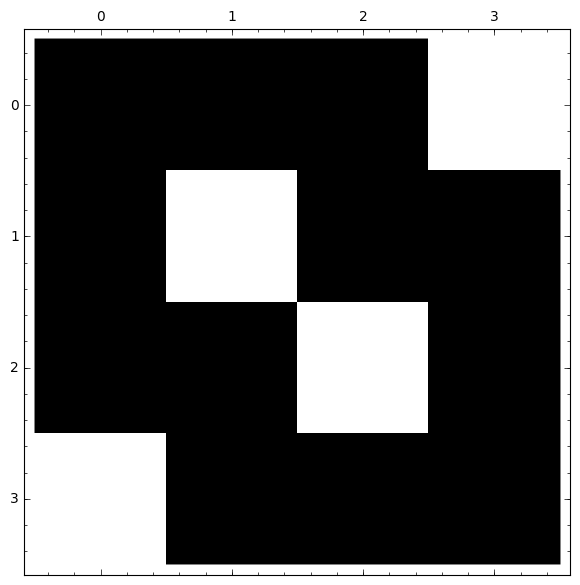
\includegraphics[width=.9\linewidth]{../matrix_plot/c2_1_bent_cayley_graph_index_matrix.png}
  \captionof{figure}{$[f_{2,1}]$: 2 extended Cayley classes, 2 General Linear classes}
  \label{fig:c2_1_bent_cayley_graph_index_matrix}
\end{minipage}
\end{figure}
\end{frame}

\begin{frame}
\frametitle{For 4 dimensions: ET class $[f_{4,1}]$}

One extended affine class, containing the extended translation class $[f_{4,1}]$, where
$f_{4,1}(x) := x_0 x_1 + x_2 x_3$.

\begin{figure}
\centering
\begin{minipage}{.48\textwidth}
  \centering
  \includegraphics[width=.9\linewidth]{../matrix_plot/c4_1_bent_cayley_graph_index_matrix.png}
  \captionof{figure}{$[f_{4,1}]$: 2 extended Cayley classes, 2 General Linear classes}
  \label{fig:c4_1_bent_cayley_graph_index_matrix}
\end{minipage}
\end{figure}
\end{frame}

\end{colortheme}

\begin{colortheme}{seagull}

\begin{frame}
\frametitle{For 6 dimensions: ET classes}

Four extended affine classes, containing the following extended translation classes:

\begin{align*}
\def\arraystretch{1.2}
\begin{array}{|cl|}
\hline
\text{Class} &
\text{Representative}
\\
\hline
\,[f_{6,1}] & f_{6,1} :=
\begin{array}{l}
x_{0} x_{1} + x_{2} x_{3} + x_{4} x_{5}
\end{array}
\\
\,[f_{6,2}] & f_{6,2} :=
\begin{array}{l}
x_{0} x_{1} x_{2} + x_{0} x_{3} + x_{1} x_{4} + x_{2} x_{5}
\end{array}
\\
\,[f_{6,3}] & f_{6,3} :=
\begin{array}{l}
x_{0} x_{1} x_{2} + x_{0} x_{1} + x_{0} x_{3} + x_{1} x_{3} x_{4} + x_{1} x_{5}
\\
 +\, x_{2} x_{4} + x_{3} x_{4}
\end{array}
\\
\,[f_{6,4}] & f_{6,4} :=
\begin{array}{l}
x_{0} x_{1} x_{2} + x_{0} x_{3} + x_{1} x_{3} x_{4} + x_{1} x_{5} + x_{2} x_{3} x_{5}
\\
 +\, x_{2} x_{3} + x_{2} x_{4} + x_{2} x_{5} + x_{3} x_{4} + x_{3} x_{5}
\end{array}
\\
\hline
\end{array}
\end{align*}
\slidecite{Rothaus 1976; Tokareva 2015}
\end{frame}

\end{colortheme}

\begin{colortheme}{jubata}

\begin{frame}
\frametitle{ET class $[f_{6,1}]$}
\begin{figure}
\centering
\begin{minipage}{.48\textwidth}
  \centering
  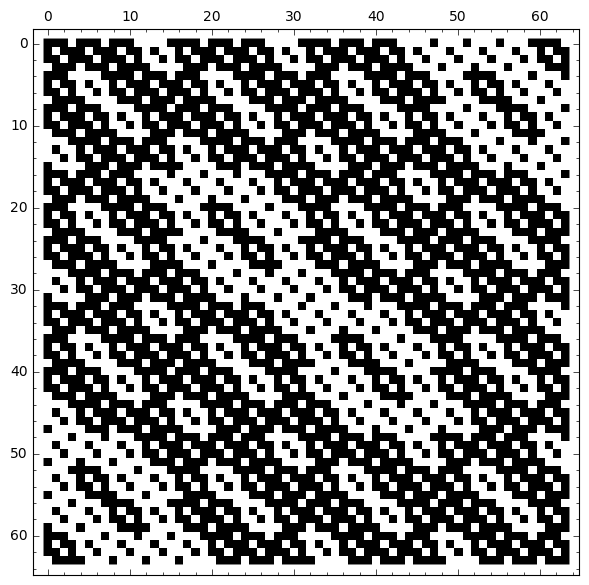
\includegraphics[width=.9\linewidth]{../matrix_plot/c6_1_bent_cayley_graph_index_matrix.png}
  \captionof{figure}{$[f_{6,1}]$: 2 extended Cayley classes, ~2 General Linear classes}
  \label{fig:6_1_bent_cayley_graph_index_matrix}
\end{minipage}
\end{figure}
\end{frame}
\begin{frame}
\frametitle{ET class $[f_{6,2}]$}
\begin{figure}
\centering
\begin{minipage}{.48\textwidth}
  \centering
  \includegraphics[width=.9\linewidth]{../matrix_plot/with_colorbar/c6_2_bent_cayley_graph_index_matrix.png}
  \captionof{figure}{$[f_{6,2}]$: 3 extended Cayley classes}
  \label{fig:6_2_bent_cayley_graph_index_matrix}
\end{minipage}
\begin{minipage}{.48\textwidth}
  \centering
  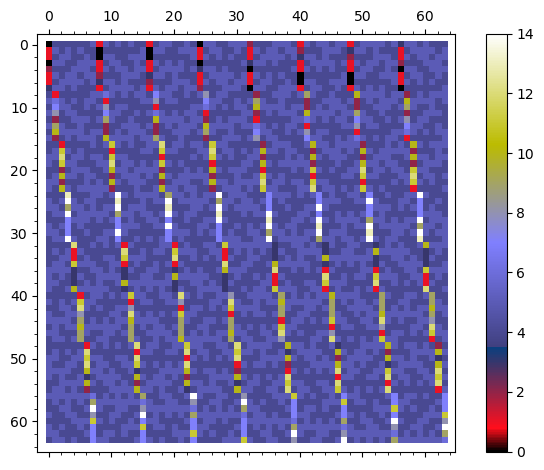
\includegraphics[width=.9\linewidth]{../matrix_plot/with_colorbar/c6_2_general_linear_class_index_matrix.png}
  \captionof{figure}{$[f_{6,2}]$: 15 General Linear classes}
  \label{fig:6_2_general_linear_class_index_matrix}
\end{minipage}
\end{figure}
Since $f_{6,1} \equiv f_{6,2}$, the Cayley graph for extended Cayley class 0 is isomorphic to the Cayley graph for class 0 of $[f_{6,1}]$.
\end{frame}
\begin{frame}
\frametitle{ET classes $[f_{6,3}]$ and $[f_{6,4}]$}
\begin{figure}
\centering
\begin{minipage}{.48\textwidth}
  \centering
  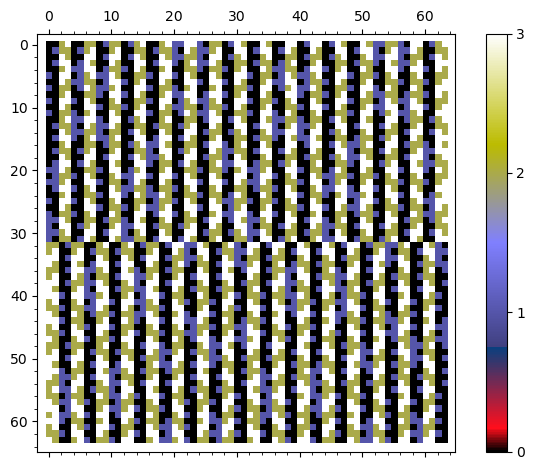
\includegraphics[width=.9\linewidth]{../matrix_plot/with_colorbar/c6_3_bent_cayley_graph_index_matrix.png}
  \captionof{figure}{$[f_{6,3}]$: 4 extended Cayley classes, ~4 General Linear classes}
  \label{fig:6_3_bent_cayley_graph_index_matrix}
\end{minipage}
\begin{minipage}{.48\textwidth}
  \centering
  \includegraphics[width=.9\linewidth]{../matrix_plot/with_colorbar/c6_4_bent_cayley_graph_index_matrix.png}
  \captionof{figure}{$[f_{6,4}]$: 3 extended Cayley classes, ~3 General Linear classes}
  \label{fig:6_4_bent_cayley_graph_index_matrix}
\end{minipage}
\end{figure}
\end{frame}
\end{colortheme}


\section{Source code, references, acknowledgements}

\begin{colortheme}{jubata}

\begin{frame}[fragile]
\frametitle{Preprint, source code and documentation}
Preprint: Paul Leopardi, Classifying bent functions by their Cayley graphs,  arXiv:1705.04507 [math.CO]. Revised, December, 2023.

~

CoCalc: Public worksheets, Sage and Python source code
\begin{verbatim}
http://tinyurl.com/Boolean-Cayley-graphs
\end{verbatim}

~

GitHub: Sage and Python source code
\begin{verbatim}
https://github.com/penguian/Boolean-Cayley-graphs
\end{verbatim}

~

SourceForge: Documentation
\begin{verbatim}
https://boolean-cayley-graphs.sourceforge.io/
\end{verbatim}
\end{frame}
\begin{frame}
\frametitle{References (1)}
\small{}
\newcounter{enumisave}
\begin{enumerate}
 \item
A.~Bernasconi and B.~Codenotti.
Spectral analysis of {Boolean} functions as a graph eigenvalue problem.
{\em IEEE Transactions on Computers}, 48(3):345--351, (1999).
 \item
A.~Braeken.
{\em Cryptographic Properties of Boolean Functions and S-Boxes}.
{PhD} thesis, Katholieke Universiteit Leuven, Belgium, (2006).
 \item
A.~Brouwer, A.~Cohen, and A.~Neumaier.
{\em Distance-Regular Graphs}.
Ergebnisse der Mathematik und Ihrer Grenzgebiete, vol. 18.
Berlin, Heidelberg, [Germany] : Springer-Verlag, (1989).
 \item
L.~Budaghyan, C.~Carlet, and A.~Pott.
New classes of almost bent and almost perfect nonlinear polynomials.
{\em IEEE Transactions on Information Theory}, 6;52(3):1141-52 (2006).
\setcounter{enumisave}{\value{enumi}}
\end{enumerate}
\end{frame}

\begin{frame}
\frametitle{References (2)}
\small{}
\begin{enumerate}
\setcounter{enumi}{\value{enumisave}}
 \item
J.~F. Dillon.
{\em Elementary {Hadamard} Difference Sets}.
PhD thesis, University of Maryland College Park, Ann Arbor, USA,
  (1974).
 \item
O.~S. Rothaus.
On ``bent'' functions.
{\em Journal of Combinatorial Theory, Series A}, 20(3):300--305,
  (1976).
 \item
N.~Tokareva.
{\em Bent functions: results and applications to cryptography}.
Academic Press, (2015).
\end{enumerate}

\end{frame}
\begin{frame}
\frametitle{Acknowledgements}
%\begin{center}
Robin Bowen,
An Braeken,
Nathan Clisby,
Robert Craigen,
Joanne Hall,
David Joyner,
Philippe Langevin,
Matthew Leingang,
William Martin,
Padraig {\'O} Cath{\'a}in,
Judy-anne Osborn,
Dima Pasechnik,
William Stein,
Natalia Tokareva, and
Sanming Zhou.

~

Australian National University. University of Newcastle, Australia. University of Melbourne.
Australian Government - Bureau of Meteorology.
National Computational Infrastructure. ACCESS-NRI.

~

SageMath, CoCalc, Bliss, Nauty, MPI4py, SQLite3, DB Browser for SQLite, PostgreSQL, Psycopg2.
%\end{center}
\end{frame}

\end{colortheme}

\end{document}
